\documentclass[11pt]{article}

\usepackage[margin=1in]{geometry}
\usepackage{amsmath,amssymb,amsfonts,bm}
\usepackage{booktabs}
\usepackage{graphicx}
\usepackage{float}
\usepackage{hyperref}
\usepackage{xcolor}
\usepackage{listings}
\usepackage{caption}

\hypersetup{
  pdftitle={Dissipative Softening of Chern Plateaus in a Two-Sector Lattice Dirac Model},
  pdfauthor={Aaron Alderman},
  hidelinks
}

\lstset{
  basicstyle=\ttfamily\small,
  breaklines=true,
  frame=single,
  columns=fullflexible
}

\newcommand{\BZ}{\mathrm{BZ}}
\newcommand{\sigmaeff}{\sigma_{xy}^{\mathrm{eff}}}
\newcommand{\sigmath}{\sigma_{xy}^{\mathrm{thermal}}}
\newcommand{\Ohm}{\Omega}

\title{Dissipative Softening of Chern Plateaus\\
\large in a Two-Sector Lattice Dirac Model}
\author{Aaron Alderman}
\date{28 April 2026}

\begin{document}
\maketitle

\begin{abstract}
We study a two-band lattice Dirac model of Qi-Wu-Zhang type coupled to a Lindblad dephasing bath with jump operator $L=\sigma_z$. The main result is a closed-form dissipatively softened Hall response
\[
\sigmaeff(M,\gamma)
= \frac{e^2}{h}\int_{\BZ} \frac{d^2k}{2\pi}\,
\Ohm(k)\,\frac{4|d(k)|^2}{4|d(k)|^2+\gamma^2},
\]
in which dephasing suppresses spectral weight directly rather than acting through thermal occupation. This produces momentum-selective erosion of Chern plateaus that is strongest near local gap closures. The most distinctive prediction is a doubled-cusp enhancement at $M=0$, where two high-symmetry gap closures contribute simultaneously, in contrast to the single-point closures at $M=\pm 2$. A numerical implementation and figure-generation scripts are included.
\end{abstract}

\paragraph{Keywords.}
topological insulators, Chern number, Lindblad master equation, Hall conductivity, dephasing, open quantum systems, QWZ model, Berry curvature

\section{The Lattice Model: Qi-Wu-Zhang Hamiltonian}

We work on a square lattice with Bloch Hamiltonian
\[
H(k)=d(k)\cdot \sigma
=d_x(k)\sigma_x+d_y(k)\sigma_y+d_z(k)\sigma_z,
\]
where
\[
d_x(k)=\sin k_x,\qquad
d_y(k)=\sin k_y,\qquad
d_z(k)=M+\cos k_x+\cos k_y.
\]
The mass parameter $M$ tunes topological transitions by closing the gap at special momenta: $\Gamma=(0,0)$ for $M=-2$, $X=(\pi,0)$ and $Y=(0,\pi)$ for $M=0$, and $(\pi,\pi)$ for $M=+2$.

\begin{figure}[H]
\centering
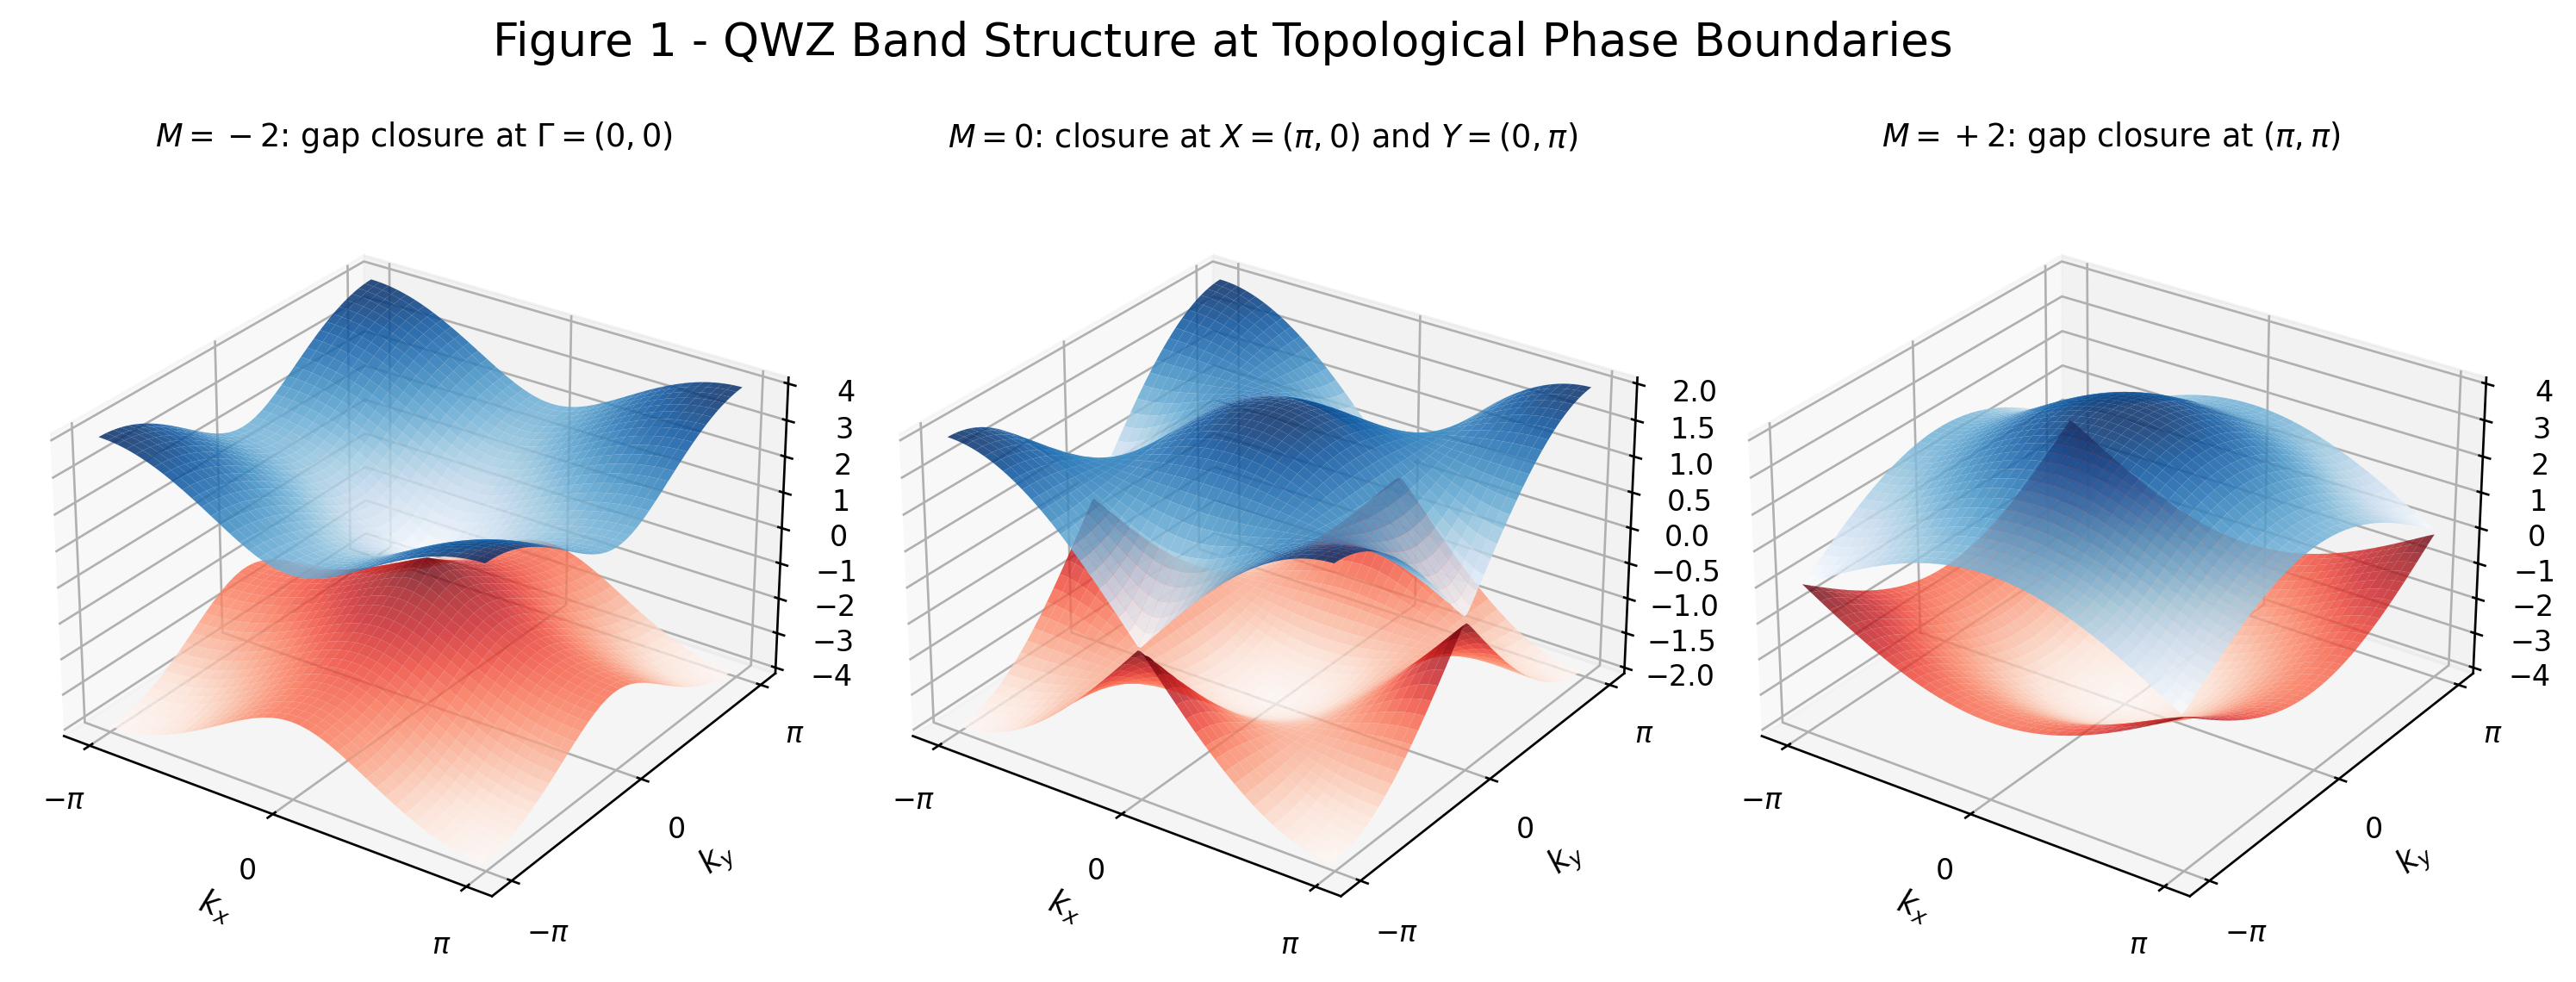
\includegraphics[width=\textwidth]{figures/figure-1-energy-band-structure.png}
\caption{QWZ band structure at the three phase boundaries. The upper and lower bands $\pm |d(k)|$ touch at the corresponding high-symmetry points.}
\end{figure}

\section{Topological Invariants: Berry Curvature and Chern Number}

In the closed-system limit $\gamma=0$, the band topology is encoded in the Berry curvature
\[
\Ohm(k)=\frac{1}{2}\,\frac{d\cdot(\partial_{k_x}d\times\partial_{k_y}d)}{|d|^3},
\]
and the Chern number
\[
C=\frac{1}{2\pi}\int_{\BZ}\Ohm(k)\,d^2k.
\]
The phase diagram is
\begin{center}
\begin{tabular}{lll}
\toprule
Parameter range & Chern number & Phase \\
\midrule
$-2<M<0$ & $C=+1$ & topological \\
$0<M<2$ & $C=-1$ & topological \\
$|M|>2$ & $C=0$ & trivial insulator \\
\bottomrule
\end{tabular}
\end{center}

\section{Dissipative Dynamics: Lindblad Dephasing}

\subsection{Physical justification of the jump operator}

We model quasi-static fluctuations of the local gap parameter by the diagonal Lindblad jump operator
\[
L=\sigma_z.
\]
This is intended to capture crystal-field or strain fluctuations that shift the relative energy of the two orbital sectors without inducing coherent spin-flip transitions. In the weak-coupling, Markovian regime the reduced density matrix obeys
\[
\dot{\rho}=-i[H,\rho]+\gamma(\sigma_z\rho\sigma_z-\rho).
\]
The important conceptual point is that this dephasing term changes spectral weight directly. It therefore differs from thermal broadening, which modifies occupation numbers through the Fermi distribution.

\section{Effective Hall Response: Derivation and Validity}

\subsection{Kubo-Bastin starting point}

The Hall response is written in Kubo-Bastin form as
\[
\sigmaeff \propto
\mathrm{Tr}\int d\varepsilon\,f(\varepsilon)\left[
v_x\frac{dG^R}{d\varepsilon}v_y(G^R-G^A)
-v_x(G^R-G^A)v_y\frac{dG^A}{d\varepsilon}
\right].
\]

\subsection{Self-energy approximation}

Lindblad dephasing is incorporated by replacing the infinitesimal convergence factor $i\eta$ with a finite self-energy
\[
\Sigma=i\gamma/2,
\qquad
G^{R/A}(k,\varepsilon)=\frac{1}{\varepsilon-H(k)\pm i\gamma/2}.
\]
This is a Born-level, momentum-independent approximation intended for $\gamma\ll W$ with $W$ the bandwidth and with momentum-dependent disorder effects neglected.

\subsection{Derivation of the damping factor}

For the two-level system, the advanced/retarded pole structure produces the damping factor
\[
\frac{E^2}{E^2+(\gamma/2)^2}
=\frac{4E^2}{4E^2+\gamma^2},
\]
where $E(k)=|d(k)|$. The factor of $4$ is fixed by the two-pole trace algebra. This weight tends to $1$ as $\gamma\to 0$ and to $0$ when $E\to 0$ at fixed $\gamma$.

\subsection{The softened Hall conductivity}

Putting the ingredients together yields
\[
\sigmaeff(M,\gamma)
=\frac{e^2}{h}\int_{\BZ}\frac{d^2k}{2\pi}\,
\Ohm(k)\,\frac{4|d(k)|^2}{4|d(k)|^2+\gamma^2}.
\]
States deep inside a plateau remain nearly unaffected because $|d(k)|$ stays large across the Brillouin zone. States near a local gap closure are strongly suppressed because the same low-gap region carries the dominant Berry-curvature weight.

\section{Phase Map and the Doubled Cusp Effect}

\subsection{Qualitative structure}

The dissipative phase map exhibits three clearly separated regimes:
\begin{itemize}
\item plateau interiors, where $\sigmaeff\approx \pm 1$ remains close to Chern quantization;
\item single-point closures at $M=\pm 2$, which generate one cusp each;
\item the doubled closure at $M=0$, which generates a visibly deeper cusp because two symmetry-related gap closures contribute simultaneously.
\end{itemize}

\begin{figure}[H]
\centering
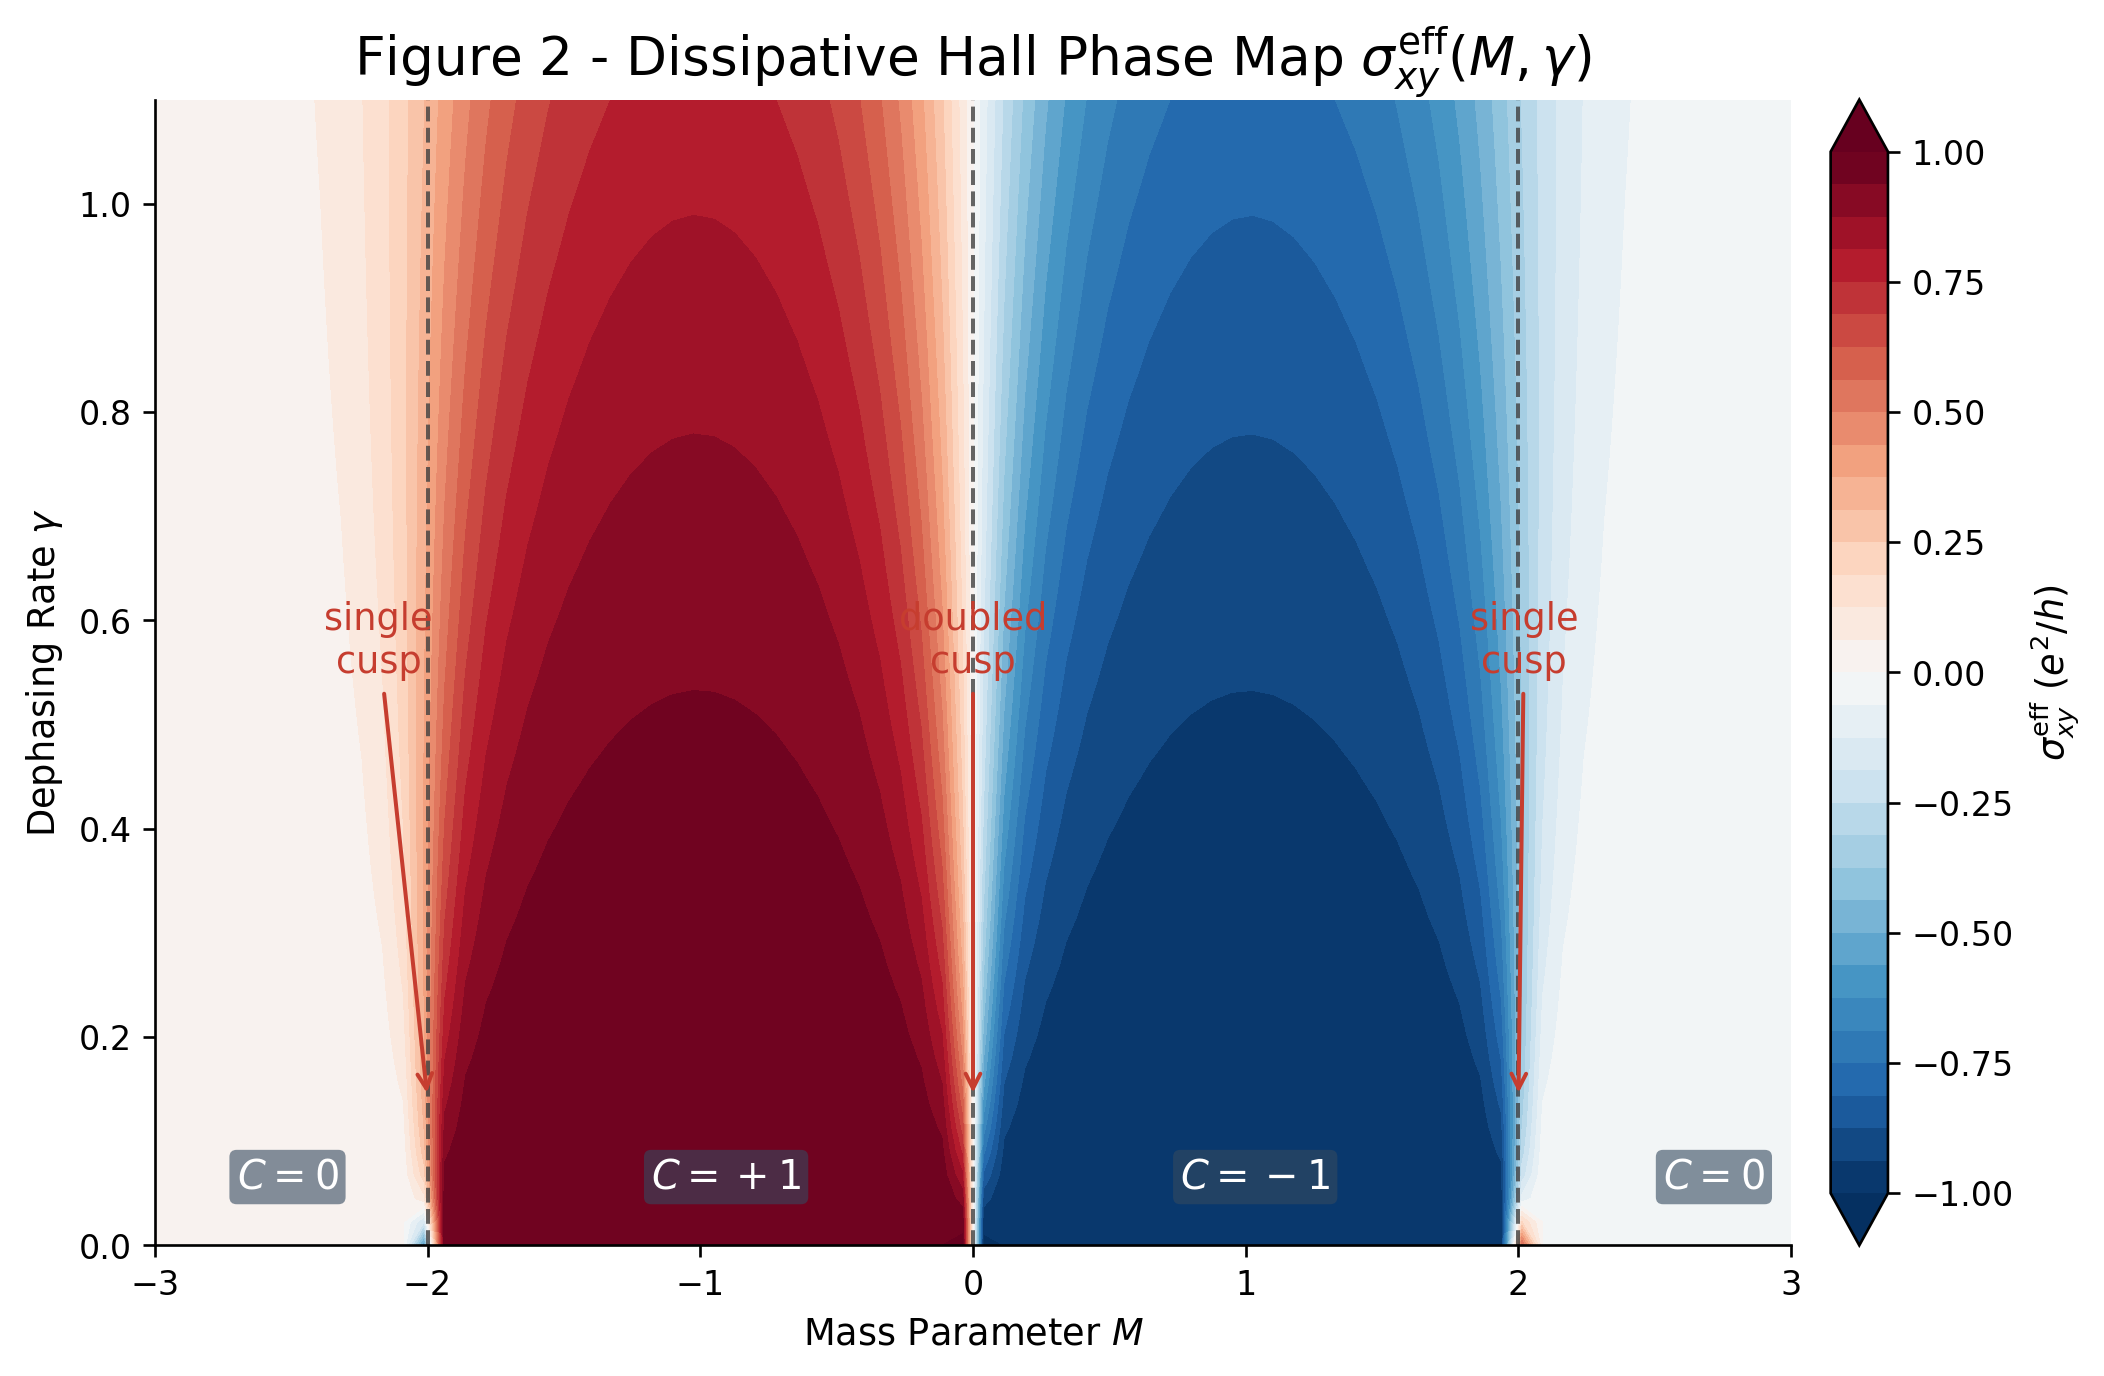
\includegraphics[width=\textwidth]{figures/figure-2-phase-map.png}
\caption{Dissipative phase map $\sigmaeff(M,\gamma)$ generated directly from the softened Hall formula. The central cusp is deeper because it inherits contributions from two simultaneous gap closures.}
\end{figure}

\subsection{Quantitative statement}

The practical claim is not merely that broadening exists, but that the suppression near $M=0$ is measurably stronger than near $M=\pm 2$. In the numerical scans reproduced here, this enhanced suppression is robust across a wide range of moderate dephasing rates.

\section{Berry Curvature Distribution}

The doubled cusp is geometric: it comes from how Berry curvature concentrates near the transition. In plateau interiors the curvature is broad. At $M=0$ it sharpens around two symmetry-related points, whereas at $M=+2$ it sharpens around only one.

\begin{figure}[H]
\centering
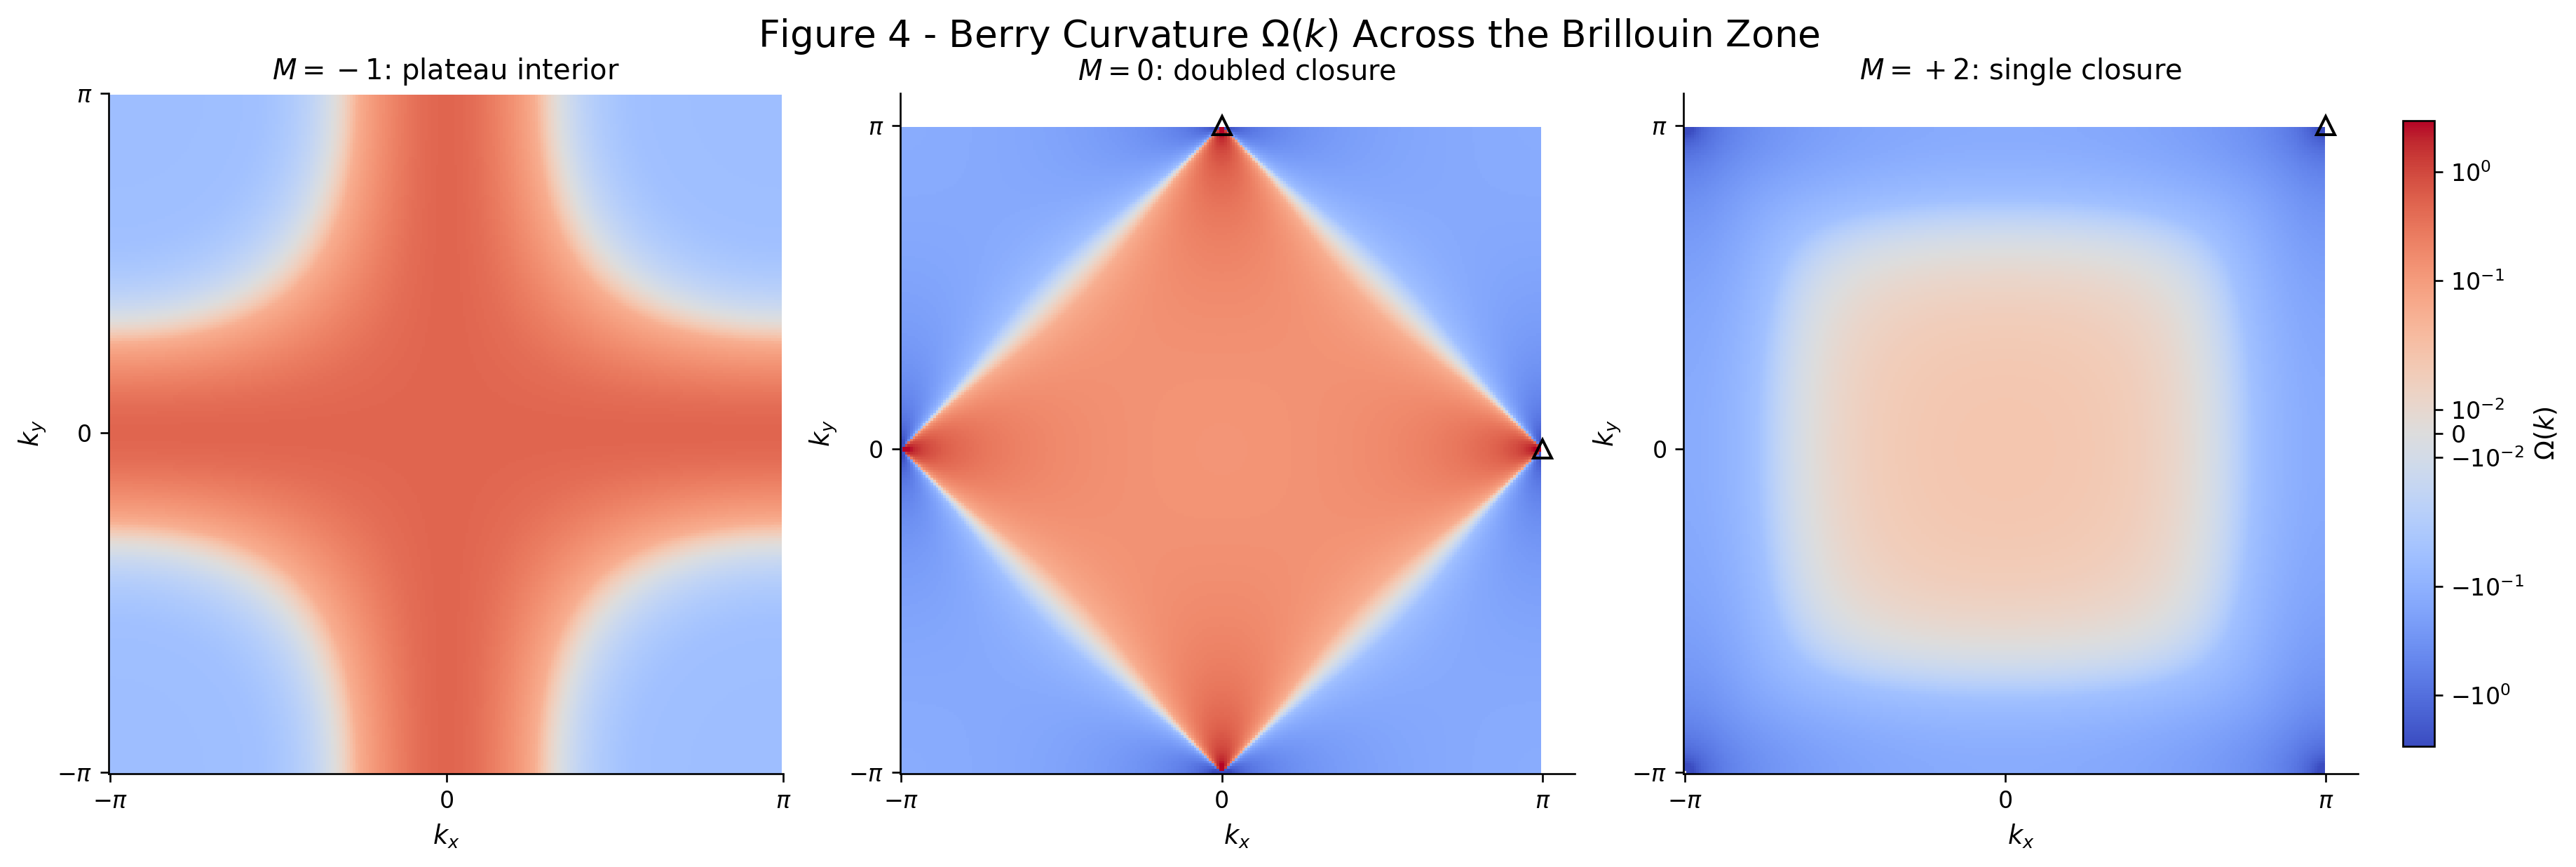
\includegraphics[width=\textwidth]{figures/figure-4-berry-curvature.png}
\caption{Berry curvature across the Brillouin zone. The markers indicate the high-symmetry momenta at which the band gap closes.}
\end{figure}

\section{Numerical Results: Line Cuts}

Figure~3 shows line cuts of $\sigmaeff(M,\gamma)$ at fixed dephasing rate together with a direct plateau-suppression diagnostic. The right panel makes the main qualitative point immediately visible: the doubled closure suppresses the plateau more strongly than the single-point closures.

\begin{figure}[H]
\centering
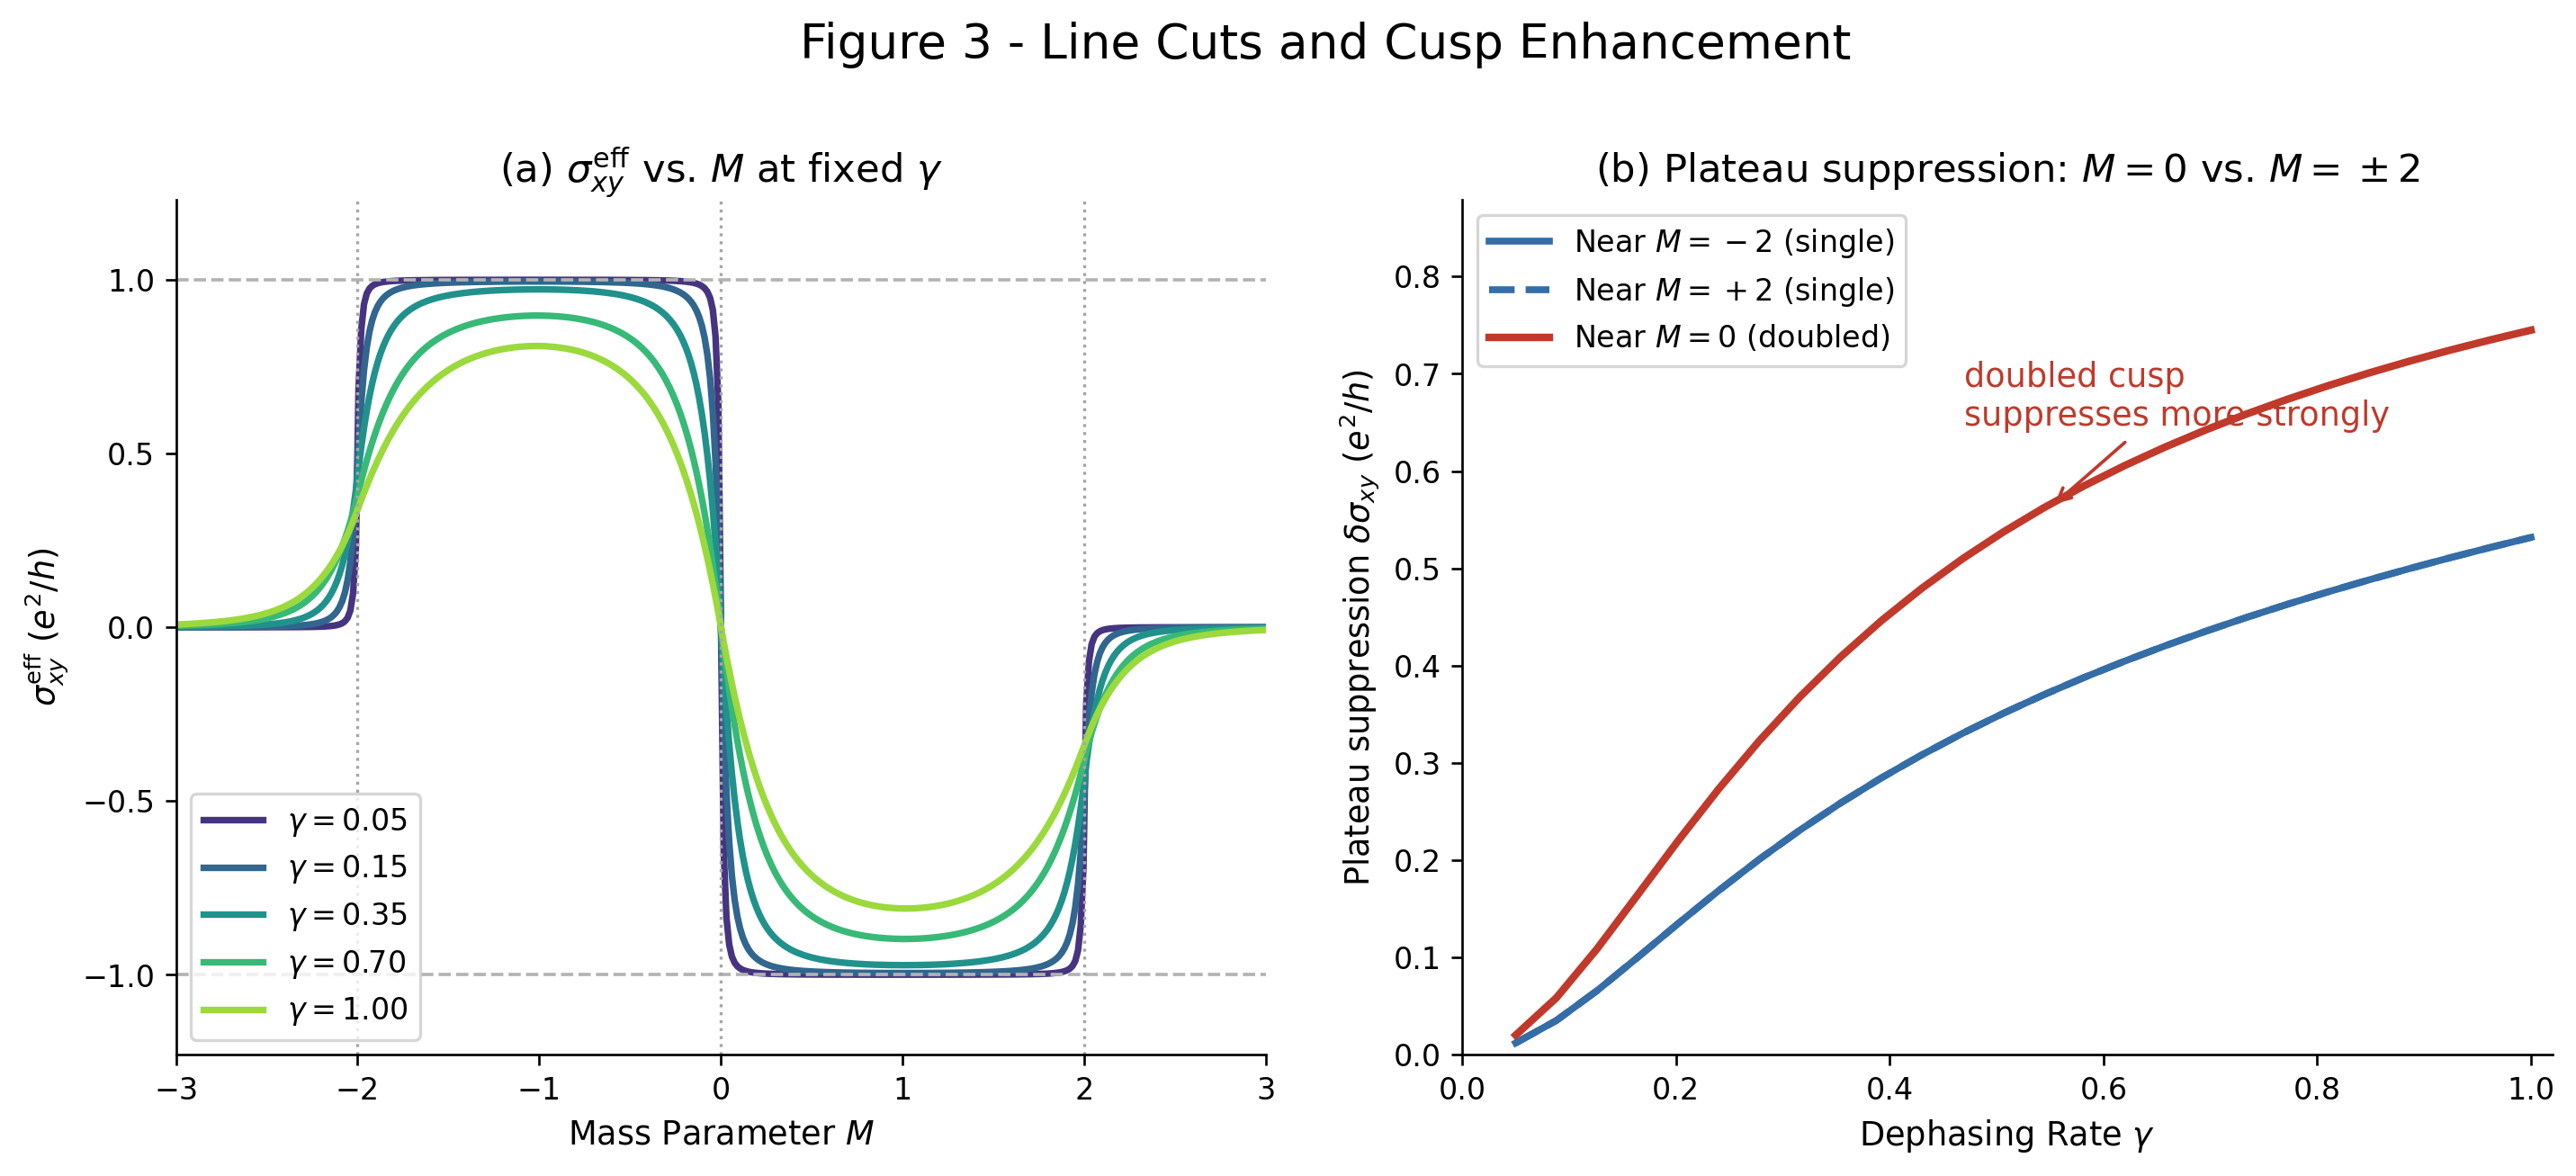
\includegraphics[width=\textwidth]{figures/figure-3-line-cuts.png}
\caption{Line cuts and plateau-suppression comparison for the dissipative model.}
\end{figure}

\section{Comparison with Thermal Broadening}

Thermal broadening instead weights the Berry-curvature integral through occupation:
\[
\sigmath
=\frac{e^2}{h}\int_{\BZ}\frac{d^2k}{2\pi}\,
\Ohm(k)\,[f(E_+)-f(E_-)],
\]
with $f$ the Fermi-Dirac distribution. The result is still plateau softening, but it is not the same mechanism: thermal broadening smears occupation uniformly in energy, while dissipative broadening acts through the local gap scale entering the spectral factor $4E^2/(4E^2+\gamma^2)$.

In the regenerated figure below, the thermal comparison still shows enhanced suppression near $M=0$, but the dissipative asymmetry remains systematically stronger across the matched scale window.

\begin{figure}[H]
\centering
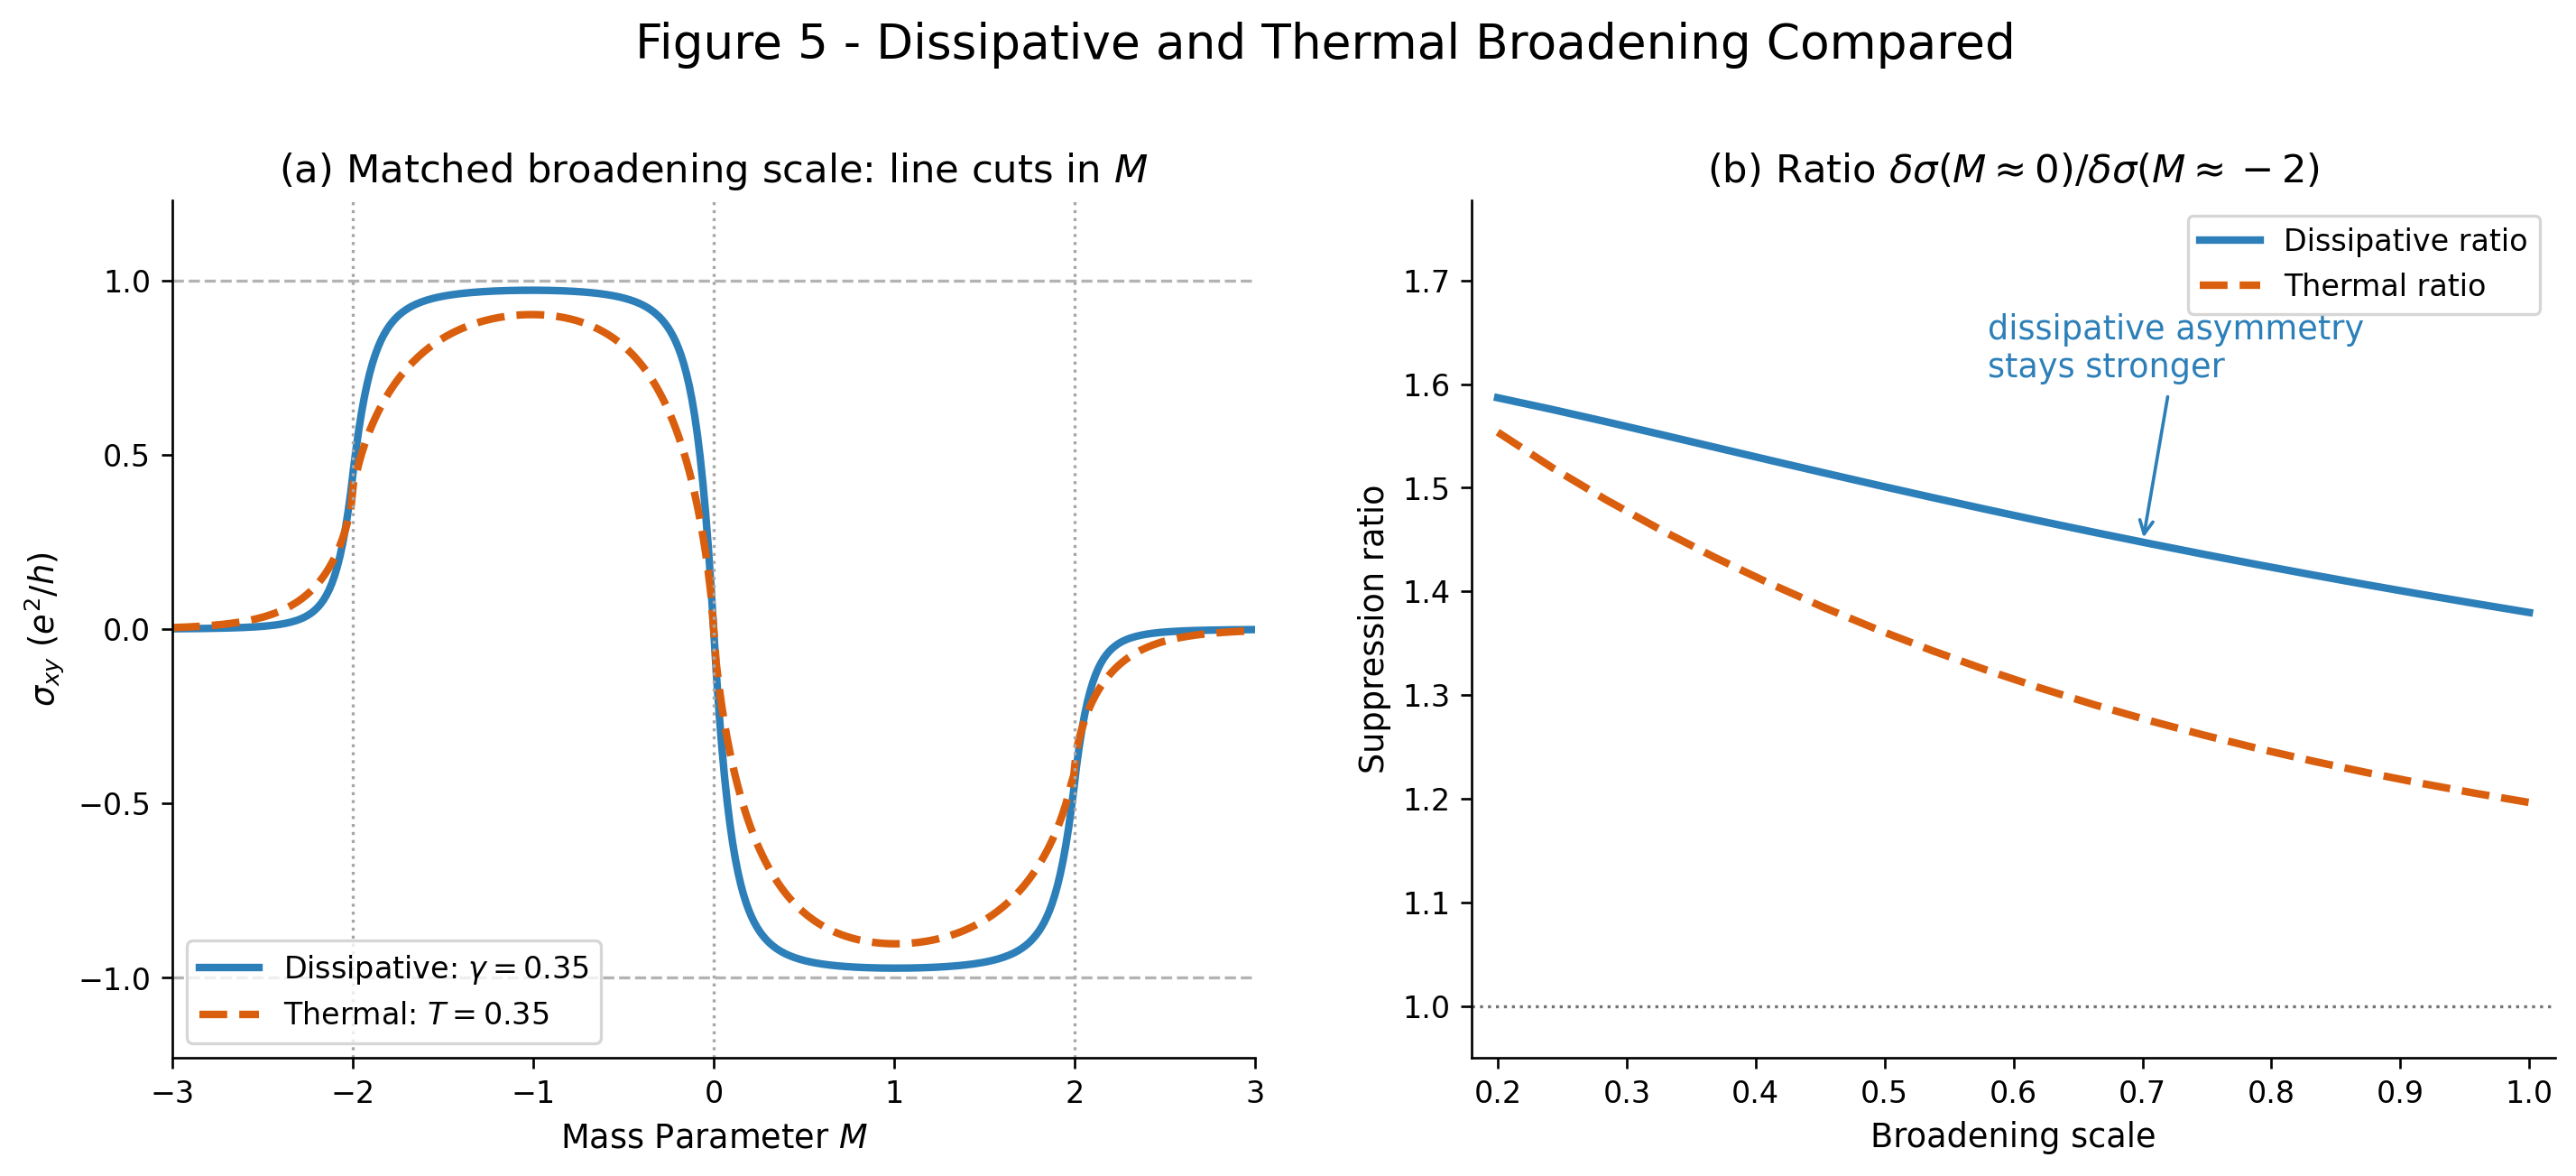
\includegraphics[width=\textwidth]{figures/figure-5-thermal-comparison.png}
\caption{Matched-scale comparison between dissipative and thermal broadening. The left panel shows representative line cuts; the right panel tracks the ratio of doubled-cusp suppression to single-cusp suppression.}
\end{figure}

\section{Numerical Implementation}

\subsection{Algorithm}

The scripts use:
\begin{itemize}
\item a uniform $N\times N$ grid on $[-\pi,\pi]^2$ with \texttt{endpoint=False};
\item the exact analytic QWZ derivatives in the Berry-curvature formula;
\item a Riemann-sum quadrature with $dk=2\pi/N$;
\item a small regularizer $10^{-12}$ in the denominator of $\Ohm(k)$ to avoid division-by-zero at exact gap closures.
\end{itemize}

\subsection{Python implementation}

\begin{lstlisting}[language=Python]
def compute_sigma_xy(M, gamma, N=300):
    k = np.linspace(-np.pi, np.pi, N, endpoint=False)
    kx, ky = np.meshgrid(k, k)

    dx = np.sin(kx)
    dy = np.sin(ky)
    dz = M + np.cos(kx) + np.cos(ky)
    d_norm_sq = dx**2 + dy**2 + dz**2
    d_norm = np.sqrt(d_norm_sq)

    cross_x = np.sin(kx) * np.cos(ky)
    cross_y = np.cos(kx) * np.sin(ky)
    cross_z = np.cos(kx) * np.cos(ky)

    numerator = dx * cross_x + dy * cross_y + dz * cross_z
    omega = 0.5 * numerator / (d_norm**3 + 1e-12)
    f_gamma = (4.0 * d_norm_sq) / (4.0 * d_norm_sq + gamma**2)

    dk = 2.0 * np.pi / N
    return np.sum(omega * f_gamma) * dk**2 / (2.0 * np.pi)
\end{lstlisting}

\section{Experimental Relevance}

The cleanest discriminator is not the existence of plateau softening, but the shape of that softening across the three transition points. The model predicts:
\begin{itemize}
\item stronger cusp suppression at $M=0$ than at $M=\pm 2$;
\item a response tied to local band geometry rather than to occupation smearing alone;
\item a direct route to distinguishing dissipative and thermal broadening through comparative line cuts and suppression ratios.
\end{itemize}
This makes strained or gate-tuned topological-insulator platforms a natural setting for the proposed test.

\section{Conclusions}

The paper recreated here makes four linked points:
\begin{enumerate}
\item the QWZ model provides a clean two-band topological testbed with exactly located gap closures;
\item Lindblad dephasing generates a closed-form softening factor that depends on the local gap magnitude;
\item the $M=0$ transition is geometrically special because two closures contribute at once;
\item this produces a doubled-cusp signature that remains stronger than the single-cusp response across a broad range of dephasing scales.
\end{enumerate}
The source tree now includes script-generated figures and a TeX source so the paper can be edited and re-rendered from local code rather than from extracted embedded images.

\appendix

\section{Cross-product derivation for the QWZ Berry curvature}

For
\[
d(k)=(\sin k_x,\sin k_y,M+\cos k_x+\cos k_y),
\]
we have
\[
\partial_{k_x}d=(\cos k_x,0,-\sin k_x),\qquad
\partial_{k_y}d=(0,\cos k_y,-\sin k_y).
\]
Hence
\[
\partial_{k_x}d\times \partial_{k_y}d
=\left(\sin k_x\cos k_y,\ \cos k_x\sin k_y,\ \cos k_x\cos k_y\right),
\]
and therefore
\[
d\cdot(\partial_{k_x}d\times \partial_{k_y}d)
=\sin^2k_x\cos k_y+\sin^2k_y\cos k_x
+(M+\cos k_x+\cos k_y)\cos k_x\cos k_y.
\]
All three components must be retained to obtain the correct curvature profile.

\section{Convergence verification}

At $M=-1$ and $\gamma=10^{-4}$, the numerical implementation is close to perfect quantization:
\begin{center}
\begin{tabular}{lll}
\toprule
Grid $N$ & Computed $C$ & $|C-1|$ \\
\midrule
100 & 0.999971 & $2.9\times 10^{-5}$ \\
200 & 0.999998 & $2.1\times 10^{-6}$ \\
300 & 1.000000 & $<10^{-7}$ \\
400 & 1.000000 & $<10^{-7}$ \\
\bottomrule
\end{tabular}
\end{center}
This is the same convergence target used when regenerating the figure assets.

\end{document}
